%!TEX root = ../thesis.tex

\chapter{Theory}\label{chapter:theory}

\section{Distributed databases}\label{sec:theory:distDbs}
This section provides overview of non-relational distributed databases with main focus on the Apache Cassandra.

%Distributed databases are .. \ref{fig:hierarchyElements}. \cite{CassandraDataStaxDocs} \cite{chandra2007PaxosMadeLive} \cite{lamport1982byzantine}

\subsection{Cassandra}
% TODO referencje do Cassandry, krotki wstep o Cassandrze
% TODO wspomnieć o LWT.
Cassandra \cite{CassandraApacheDocs} \cite{CassandraDataStaxDocs} is a high performance, extremely scalable, fault tolerant (i.e. no single point of failure), distributed post-relational database solution, which combines all the benefits of Google Bigtable \cite{chang2008bigtable} and Amazon Dynamo \cite{decandia2007dynamo}.
% to handle the types of database management needs that traditional RDBMS vendors cannot support. 

%Cassandra offers linear scale performance, which means that, for example if four nodes can handle hundred thousand 
%requests per second, then adding another four nodes results in the cluster, which can handle twice as much requests per second. Cassandra provides continous availability, due to redundancy of both data and node functions, which eliminate SPOF and provide constant uptime. 

\subsubsection{Key features}
Its key features are:
\begin{enumerate*}
\item masterless architecture,
\item linear scale performance \ref{sec:theory:cassandra:linear},
\item continuous availability,
\item flexible data model \ref{sec:theory:cassandra:datamodel},
\item multi data center support,
\item all nodes accept reads and writes,
\item Cassandra Query Language \ref{sec:theory:cassandra:cql}.
\end{enumerate*}

\subsubsection{Architecture}
Cassandra has a masterless \emph{ring} architecture, in which all nodes are equally significant, and there is no master node, therefore there is no single point of failure (SPOF). \emph{Gossip} is a scalable, distributed protocol used for inter-node communication. Cassandra uses replication, which is keeping copies of the data on multiple nodes, to also avoid SPOF during reads and writes. Replication factor -- number of nodes on which the data is stored -- is configurable per keyspace \ref{sec:theory:cassandra:datamodel}. Cassandra provides continous availability, due to redundancy of both data and node functions, which eliminate SPOF and provide constant uptime.

TODO Read path

TODO Write path

TODO Rysunek z token range i replication -> więcej o replikacji

%Architecture
% Token ring
% rysunek z klastrem

\begin{figure}[h]
	\centering
	%\subfloat[The cluster on the ring]
	%{
	\label{fig:archClusterA}
\includegraphics[height=60mm]{images/cassandra-ring.png}\hspace{10mm}
	%}
	\label{fig:archCluster}
	\caption{A cluster on the ring}
\end{figure}

\subsubsection{Data model}
\label{sec:theory:cassandra:datamodel}
Cassandra's data model is a wide-row store, which consists of tables, which reside in keyspaces\footnote{comparable to schemas in RDBMS} with rows, identified by primary keys, with up to 2 billion columns. Although data model concepts are familiar to relational ones, data modeling techniques depart from the relational modeling, since models are supposed to be highly denormalized, which provide ability to perform fast queries by reading single partition, which is the unit of the data replication in Cassandra, in order to fetch all the data the query needs without further communication with other nodes and performing joins\footnote{which do not exist in Cassandra}.

%\begin{description}
%\item[keyspace] 
%\item[table]
%\item[column]
%\item[row]
%\item[primary key]
%\end{description}

\subsubsection{Linear scale performance}
\label{sec:theory:cassandra:linear}
Cassandra offers linear scale performance, which means that, for example \ref{fig:archLinearScale} if two nodes can handle hundred thousand requests per second, then adding another two nodes results in the cluster, which can handle twice as much requests per second. 

The key principles behind linear scaling are:  data partitioning and token ranges. 
Partitioning is the assignment of the token values, which are \emph{long} values, to the keys, and more concretely to the partitioning keys of a primary key. Cassandra provides different \emph{Partitioners}, which implement different algorithms to perform such token assignment. \emph{Murmur3Partitioner} uses \emph{Murmur3} hash algorithm that provides a good distribution over the hash space, and is fast due to the fact that it does not support cryptographic properties, which are not required by Cassandra.

Each node is responsible for a token range, which is a part of the token ring. Responsibility means that a node stores the data for which the token value falls into its token range. When a new node is added, it automatically receives a token range and then the data is moved between the nodes in order to adjust to the new division of the token ring.

Correct data modeling is also an important aspect of the linear scalability, since partitioning keys of tables have to be designed in a way that provides high cardinality of the keys. Otherwise part of the cluster starts to collect more data than its storage capabilities, and it will fail. 


\begin{figure}[H]
  \centering  
  % TODO źródło?
  % Źródło http://docs.datastax.com/en/cassandra/2.1/cassandra/images/intro_cassandra.png
  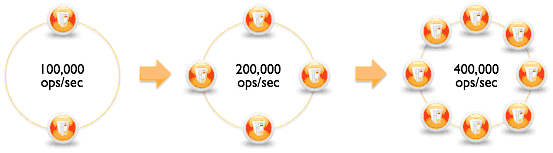
\includegraphics[width=\textwidth]{images/cassandra-linear-scalability.png}\hspace{10mm}
  \label{fig:archLinearScale}
  \caption{The linear scalability from 100k to 200k requests per second}
\end{figure}


%Linear scale performance is provided by even assignment of token ranges of the token ring to the nodes in the cluster combined with data \emph{partitioning} -- which is assigning a token values to the keys -- that evenly distributes the data around the cluster. When a new node is added to the cluster, it automatically 


\subsubsection{Cassandra Query Language}
\label{sec:theory:cassandra:cql}
Cassandra Query Language (CQL) is the query language, similar in syntax to SQL, but provides only limited functionality compared to SQL, as there are no joins, inner queries, nor aggregations. CQL provides select, insert, update and delete statements. Select statement's \emph{where} clause supports equality condition on the partition key columns and restrictions such as: IN, =, >, >=, <= and < on the clustering columns. Columns, which are not part of the primary key cannot be restricted in the \emph{where} clause. Listing \ref{lst:cqlSelect} shows two examples of select statements, first with equality restriction on the partition key column \emph{user_id}, second with equality restrictions on the partition key columns: \emph{cluster}, \emph{date}, \emph{datacenter}, and range restrictions on the clustering key columns: \emph{hour} and \emph{minute}.
%Cassandra uses binary protocol named Cassandra Query Language (CQL). In order to do anything with database, we need to use a driver that speaks binary protocol. 

\begin{lstlisting}[style=outcode,label={lst:cqlSelect},caption={Examples of CQL select statements}]
SELECT user_name, user_email 
FROM app.users 
WHERE user_id = 10123;
    
SELECT * FROM app.requests
 WHERE cluster = 'cluster1'
 AND date = '2015/06/05'
 AND datacenter = 'EU_NORTH'
 AND (hour, minute) >= (12, 0) AND (hour, minute) <= (15, 30);
\end{lstlisting}

 
\subsubsection{Use cases}
Cassandra is a general purpose non-relational database, however there are areas in which Cassandra excels over other databases:
\begin{enumerate*}
\item internet of things applications - Cassandra is able to consume large quantity of incoming data\footnote{depends on cluster size} from devices, sensors and similar internet connected devices,
%\item E-commerce - durable shopping cart protection combined with fast product catalog browsing
%\item Messaging - Cassandra serves as the database for mobile phone applications
\item data analytics - Cassandra provides storage with fast access to the data for analysis. Apache Spark, which is an engine to perform large-scale data processing \cite{ApacheSpark} supports Cassandra, as one of its data sources, therefore Cassandra provides data storage for analytics and also stores results of the analysis done in Spark,
\item storage of time series data - Cassandra's fast writes, wide-rows and ability to read only particular data ranges are well suited for time series based applications, because such data fits natively into the data model.
\end{enumerate*} 

\subsubsection{Transactions}
Cassandra does not provide ACID compliant transactions, but it offers Light Weight Transactions, which offer a degree of transactionality limited to the scope of single partition, therefore to the single primary key\footnote{concretely to the partitioning part of the key in terms of the complex key}. Section \ref{sec:theory:transactions:lwt} provides more on this subject in comparison to other distributed transactions. 

\subsubsection{Compared to RDBMS}
Tablelka + referencja

\subsubsection{Eventual consistency}\label{sec:theory:eventualConsistency}
In terms of CAP \cite{brewer2000towards} \cite{Brewer:2012ba} Cassandra is the \emph{AP} database with eventual consistency, which means that over time the data becomes consistent on all nodes, but there are no guarantees about time it takes. Cassandra uses techniques such as: \begin{enumerate*} 
\item \emph{hinted handoff} - stores a message for the currently unavailable replica about the modification and sends it to the replica when it comes back up \cite{CassandraHintedHandoff},  
\item \emph{read repairs} - detects inconsistency in the data during read and repairs it by sending a message with the data \cite{CassandraReadRepair},  \end{enumerate*} to pro-actively reduce incosistency in the data during normal operations.

\subsection{MarkLogic}
MarkLogic is a NoSql database with the document-centric schema-agnostic data model \cite{markLogicDataModel} and support of ACID transactions \cite{markLogicAcid}.
MarkLogic has native support for formats such as JSON, XML and RDF. ACID transactions are implemented by the means of multi-version concurrency control (MVCC) and locking. In an MVCC system, changes are tracked with a timestamp number on each document. 
The database uses these timestamps to ensure that all users see consistent data. 
Transaction has to acquire write locks on all of the updated documents and read locks on all of the queried documents in order to complete evaluation. Acquired locks are held until the transaction ends, which prevents other transactions from updating the read locked document and ensures a read-consistent view of the document. 
Deadlocks might happen, but are detected by database, and are dealt with by aborting one or the other request and retrying it later \cite{markLogicUnderstandingTransactions}.

% Bazy które wspierają jakieś transakcje
% ACID transactions

\subsection{FoundationDB}
FoundationDB is a NoSql database with ACID compliant transactions, strong scalability and SQL querying capabilities.
Its core data model is a ordered key-value store. The ordering property increases efficiency of range reads. It also supports document store and relational DBMS as layers on top of the core model.  The database scaled up to $14,4$ million random writes per second. FoundationDB was acquired by Apple \cite{foundationDbAcquired} and since then no information is available. Its website is shutdown, documentation is not accessible nor downloads of the database.
% Było, miało transakcje, zostało wchłonięte przez Apple i znikneło z Internetu

% TODO inne rozproszone bazy z transakcjami, takie jak Cassandra

\subsection{Distributed relational databases}
% TODO wspomnieć coś o tym, napisać, że jest. Może porównać z Cassandrą






\section{Transactions}\label{sec:theory:transactions}
Transactions in RDBMS

% TODO organizacja rozdziału, czy paxos powinien mieć pełny opis, czy tylko referencja? 
\subsection{ACID}

\subsection{2 phase commit}

\section{Distributed transactions}
% TODO rozrysować co czym jest, Raft, Paxos -> distributed consensous algorithm
% RAMP atomic commit

% LWT (CAS) distributed transaction, compare and set with distributed consensous. Implementacja w Cassandrze.

\subsection{3 phase commit}\label{sec:theory:transactions:3pc}

\subsection{Paxos}

% TODO opisać na tyle szczegółowo żeby móc je porównać. 
% bez dokładnego schematu
% ogólny schemat, najbardziej typowy przypadek opisać, bez dowodów, bez wyników testów.
% żeby było wiadomo o co chodzi.

% po to żeby móc porównać, Paxos jest lepszy od 3PC bo (ma partycje) i źródło "dokładnie jest to opisane tu i tam"
% ma wynikać z jakiego powodu jest lepszy


%  Paxos, Raft, 3PC opisane na jednym poziomie szczegółowości

% żeby do zrozumienia pracy nie trzeba było zaglądać gdzieś indziej.


\subsection{Raft}
% TODO napisać jakie to są guarantees
\emph{Raft} algorithm offers the same guarantees, as \paxos. 
The aim of Raft designers was to create a consensus algorithm which would be more understandable to its predecessor \cite{ongaro2014search}. 
The main idea behind the algorithm is decomposition of the consensus problem into the following individual tasks:
\begin{enumerate*}
\item leader election,
\item log replication,
\item safety,
\item membership changes.
\end{enumerate*} 
%Safety property is that: if any server
%has applied a particular log entry to its state machine,
%then no other server may apply a different command for the same log index.
 Using \emph{Raft} each server is in one of three states: \begin{enumerate*} \item leader, \item follower, \item candidate \end{enumerate*}. The leader can be only one and it handles all client requests. When a follower receives a request, it has to redirect request to the leader. The candidate state is used during leader election. 
% TODO reszta opisu

 %The difference to \paxos  is that \emph{Raft} has been decomposed into independent subproblems which clearly address problems. 

% TODO %
% Napisać jak ten RAFT działa
\emph{Raft} uses \emph{Leader election}. Leader is elected for specific term. \emph{Raft} uses \emph{Log Replication} to arrive at consensus. Leader proposes new value to \emph{followers} which append value to uncommitted log. Once leader has majority of acknowledges it sends commit message. Followers receive commit message and commit value in the log. 

\emph{Raft} algorithm is visualized in \cite{raftVisual}.

\subsection{RAMP}\label{sec:theory:transactions:ramp}
\emph{Read Atomic Multi Partition} transactions \cite{Bailis:2014} is the newest algorithm among the algorithms discussed in this chapter. 
\emph{RAMP} algorithm was designed to address the requirements of the following use cases: secondary indexing, foreign key
enforcement, and materialized view maintenance.
\emph{RAMP} identifies new transaction isolation level \emph{Read Atomic}, which 
assures consistent visibility of changes made by the transaction: either all or none of each transaction's updates are seen by other transactions.
\emph{RAMP} is resilient to partial failures -- failures of part of the nodes in the cluster -- for the reason that RAMP's transaction does not contact nodes that are not affected by the transaction. 
\emph{RAMP} also guarantees \emph{synchronization independence}, which means that transactions do not stall or fail other transactions, due to the fact that reads and writes do not block each other. 

%The transaction is able to detect non-atomic partial read and repair it with additional rounds of communication with nodes. 
The key principle behind \emph{RAMP} is its ability to detect non-atomic partial read, and to repair it with additional rounds of communication with the nodes by the means of \emph{the metadata} attached to each write and \emph{multi-versioning}, which means that the data is accessible in different versions and each modification to the data creates a new version. Versions are either committed or not yet committed in which case the data can be discarded by aborting the transaction \cite[p. 6]{Bailis:2014}. 
There are three variants of \emph{RAMP} algorithm and the difference between them is the type of the metadata. \emph{RAMP-small} uses a 64 bit timestamp as the metadata and requires additional two rounds of communication when non-atomic read is detected. Other variants of \emph{RAMP} are described in \cite[p. 5]{Bailis:2014}.
\emph{RAMP} was proven to be linearly scalable with the number of nodes during trials spanning up to 100 servers \cite[p. 10]{Bailis:2014}.
%\emph{RAMP} ensures \emph{atomic visibility}: either all or none of each transaction's updates are seen by other transactions.
 
%client’s transactions cannot stall or fail another client’s transactions.
%(via \emph{synchronization independence}) 
%and provides network partition tolerance by minimized communication between servers, which means that client does not contact servers which are not directly referenced by the transaction.

% OD JACKA

%The key principle behind \emph{RAMP} is  multi-versioning with a variable but small amount of metadata per write. \emph{RAMP} transactions are linearly scalable. Scalability has been tested up to 100 servers.

\subsection{LWT}\label{sec:theory:transactions:lwt}
% TODO źródło w (more on this)
As mentioned earlier, Light Weight Transactions is the name of compare-and-swap functionality implemented in Cassandra. Internally, LWT uses the Paxos algorithm with some modifications which were aimed to prevent potential single point of failure, thus improving high availability. SPOFs may surface in case the leader fails when it is about to propose a new value (more on this…). The problem was addressed by sacrificing the standard leader election in favour of allowing any node to act as a leader, so that it can propose a value at any time. On the downside, such approach increases the risk of contention. 

One of the key requirements of Paxos protocol is storage of PaxosState - a data structure composed of the proposed value, proposed ballot, promised ballot and most recent commit. In case of LWT, the value represents the update itself along with the token of the partition key where that update should be applied. That token uniquely identifies PaxosState so that several proposals for the same partition can be associated with the same Paxos instance. 


LWT includes the following phases: \begin{enumerate*}
\item prepare,
\item get promise,
\item read row,
\item get results,
\item propose a new value,
\item acceptance,
\item broadcast commit,
\item wait for acknowledgements.
\end{enumerate*} Let us analyze each of them in the environment with 5 nodes, replication factor 3 and request to insert user named \emph{John} to \emph{users} table, but only if \emph{John} does not exist. For simplicity, \emph{users} table has only two columns: \begin{enumerate*} 
\item name -- text column and primary key, \item email -- text column. \end{enumerate*} LWT begins with a node 5 receiving request. Node 5 is then called coordinator node. The coordinator has to become the leader of paxos round identified by the token computed from partition key of \emph{users} table, thus from string value \emph{John}. To become the leader, the coordinator has to create the new ballot and send it along with the token and table name to replica nodes: node 1, node 2, node 3. Each replica has to check whether the ballot is the highest ballot it has seen, and if it is, then replica saves it in the PaxosState and responds with a promise. The leader has to wait for majority of promises before it proceeds. When majority promises, the coordinator may proceed to read the row and check the condition. The condition is that \emph{John} cannot exist, thus read has to not find any rows querying users by user name \emph{John}. Let us assume that indeed user \emph{John} did not exist, thus condition is met which allows the coordinator to propose an insert of \emph{John} with email \emph{john.doe@gmail.com} to \emph{users} table. The coordinator sends proposal message, with an insert and same ballot, to replicas and waits for acceptances. A replica saves proposed insert to PaxosState and replies with acceptance message.
When the coordinator receives majority of acceptances it broadcasts the commit message and waits for majority of acknowledgements. Upon receiving commit message a replica applies an update stored in PaxosState, thus it performs the insert of \emph{John} to \emph{users} table and acknowledges commit with a reply.

At any time during whole procedure at minority of replicas might stop responding and LWT can continue. In this case, one node can fail without affecting \emph{LWT}. If more than one node fails, then LWT is aborted. 

Also at any time the leader might lose leadership if other node does prepare with a higher ballot. In that case the coordinator has to wait, giving other leader time to complete its \lwt, and try again with new ballot.

Note that \lwt affects only limited number of nodes -- replicas of the key, thus majority is considered only at the level of replicas, not at the level of the cluster.


%1. LWT is initiated by client request: insert John if not exists
%2. Request is routed to some node X that becomes coordinator of LWT
%3. Coordinator wants to be a leader so it creates a ballot and sends prepare to replicas: node1, node2, node3. This is prepare phase.
%4. Replicas promise to not accept values from leaders who have lower ballots.
%5. Coordinator gets 3 of out 3 promises. Quorum promised to listen.
%6. Coordinator performs read: SELECT * FROM users WHERE user_id = 1
%7. Coordinator checks condition “IF NOT EXISTS”. If such row did not exist in quorum of replicas it proceeds further
%8. Coordinator, as a leader, proposes new value which is an insert to users table.
%9. All three nodes reply with accept. Quorum accepted insert.
%10. At this point, insert is an in progress proposal that has been accepted by majority of replicas. Even if coordinator crashes, once someone selects user with id=1 or retries to insert it. This proposal will get committed. Let’s assume that coordinator is well and proceeds to commit.
%11. Coordinator broadcasts commit message
%12. Replicas apply insert locally and reply with acknowledge message
%13. Coordinator receives quorum of acknowledges. LWT has been successfully completed.
%14. Coordinator responds to client: John was inserted.


%Sequence above is a happy path. At any point coordinator might lose his leadership if some other node sends prepare with higher ballot. In that case coordinator waits a bit and retries whole process again. 
%Also any replica might stop responding, which is fine as long as quorum is up and well. If quorum responds to messages, coordinator can proceed. If there is no quorum then paxos conditions are not met and LWT cannot be continue. However during normal operation is it rather rare to see many nodes down so in general LWT can successfully finish with 2 out of 3 replicas running. Note that cluster size might be much bigger, for example hundred nodes, but since replication factor N=3, only three nodes are interesting from perspective of LWT and Paxos.


\subsection{Datomic}
% TODO podejście na jeszcze wyższym poziomie abstrakcji. 
